\documentclass[11pt,a4paper]{report}
\usepackage[utf8]{inputenc}
\usepackage[T1]{fontenc}
\usepackage[spanish]{babel}
\usepackage{geometry}
\geometry{margin=2.5cm}
\usepackage{amsmath,amsfonts,amssymb}
\usepackage{booktabs,longtable,multirow}
\usepackage{graphicx}
\usepackage{hyperref}
\usepackage{cleveref}
\usepackage{siunitx}
\usepackage{caption,subcaption}
\usepackage{xcolor}
\usepackage{listings}
\usepackage{fancyhdr}
\usepackage{titlesec}
\usepackage{float}

% Colores
\definecolor{wasaffblue}{RGB}{0,82,147}
\definecolor{codebg}{RGB}{245,245,245}

% Encabezados
\pagestyle{fancy}
\fancyhf{}
\fancyhead[L]{\small\textcolor{wasaffblue}{WASAFF Consulting — Informe Técnico}}
\fancyhead[R]{\small\textcolor{wasaffblue}{CMPC/SSD — Kaeser}}
\fancyfoot[C]{\thepage}
\renewcommand{\headrulewidth}{0.4pt}

% Títulos de sección
\titleformat{\chapter}[display]{\normalfont\huge\bfseries\color{wasaffblue}}{\chaptertitlename\ \thechapter}{20pt}{\Huge}
\titleformat{\section}{\normalfont\Large\bfseries\color{wasaffblue}}{\thesection}{1em}{}
\titleformat{\subsection}{\normalfont\large\bfseries\color{wasaffblue!80}}{\thesubsection}{1em}{}

% Listings
\lstset{
  backgroundcolor=\color{codebg},
  basicstyle=\ttfamily\small,
  breaklines=true,
  frame=single,
  numbers=left,
  numberstyle=\tiny\color{gray},
  keywordstyle=\color{wasaffblue}\bfseries,
  commentstyle=\color{gray}\itshape,
}

\begin{document}

% =================== PORTADA ===================
\begin{titlepage}
\centering
\vspace*{2cm}
{\Huge\bfseries\textcolor{wasaffblue}{Sistema de Recuperación de Calor}}\\[0.3cm]
{\Huge\bfseries\textcolor{wasaffblue}{de Aceite de Compresores}}\\[0.3cm]
{\LARGE\bfseries\textcolor{wasaffblue}{CMPC Planta Santa Fe}}\\[1.5cm]
{\Large\textit{Informe Técnico de Ingeniería de Detalle}}\\[0.5cm]
{\large Nivel de Servicio: Nivel 2 (MSc) — Modelación Numérica Avanzada}\\[2cm]
\rule{\textwidth}{0.5pt}\\[0.5cm]
{\large\textbf{Cliente:} Kaeser Compresores Chile SpA / CMPC Planta Santa Fe}\\[0.3cm]
{\large\textbf{Consultor:} WASAFF Consulting}\\[0.3cm]
{\large\textbf{Proyecto:} 2026\_Kaeser\_RecuperacionCalorCMPC}\\[0.3cm]
{\large\textbf{Fecha:} Mayo 2026}\\[1cm]
\rule{\textwidth}{0.5pt}\\[1cm]
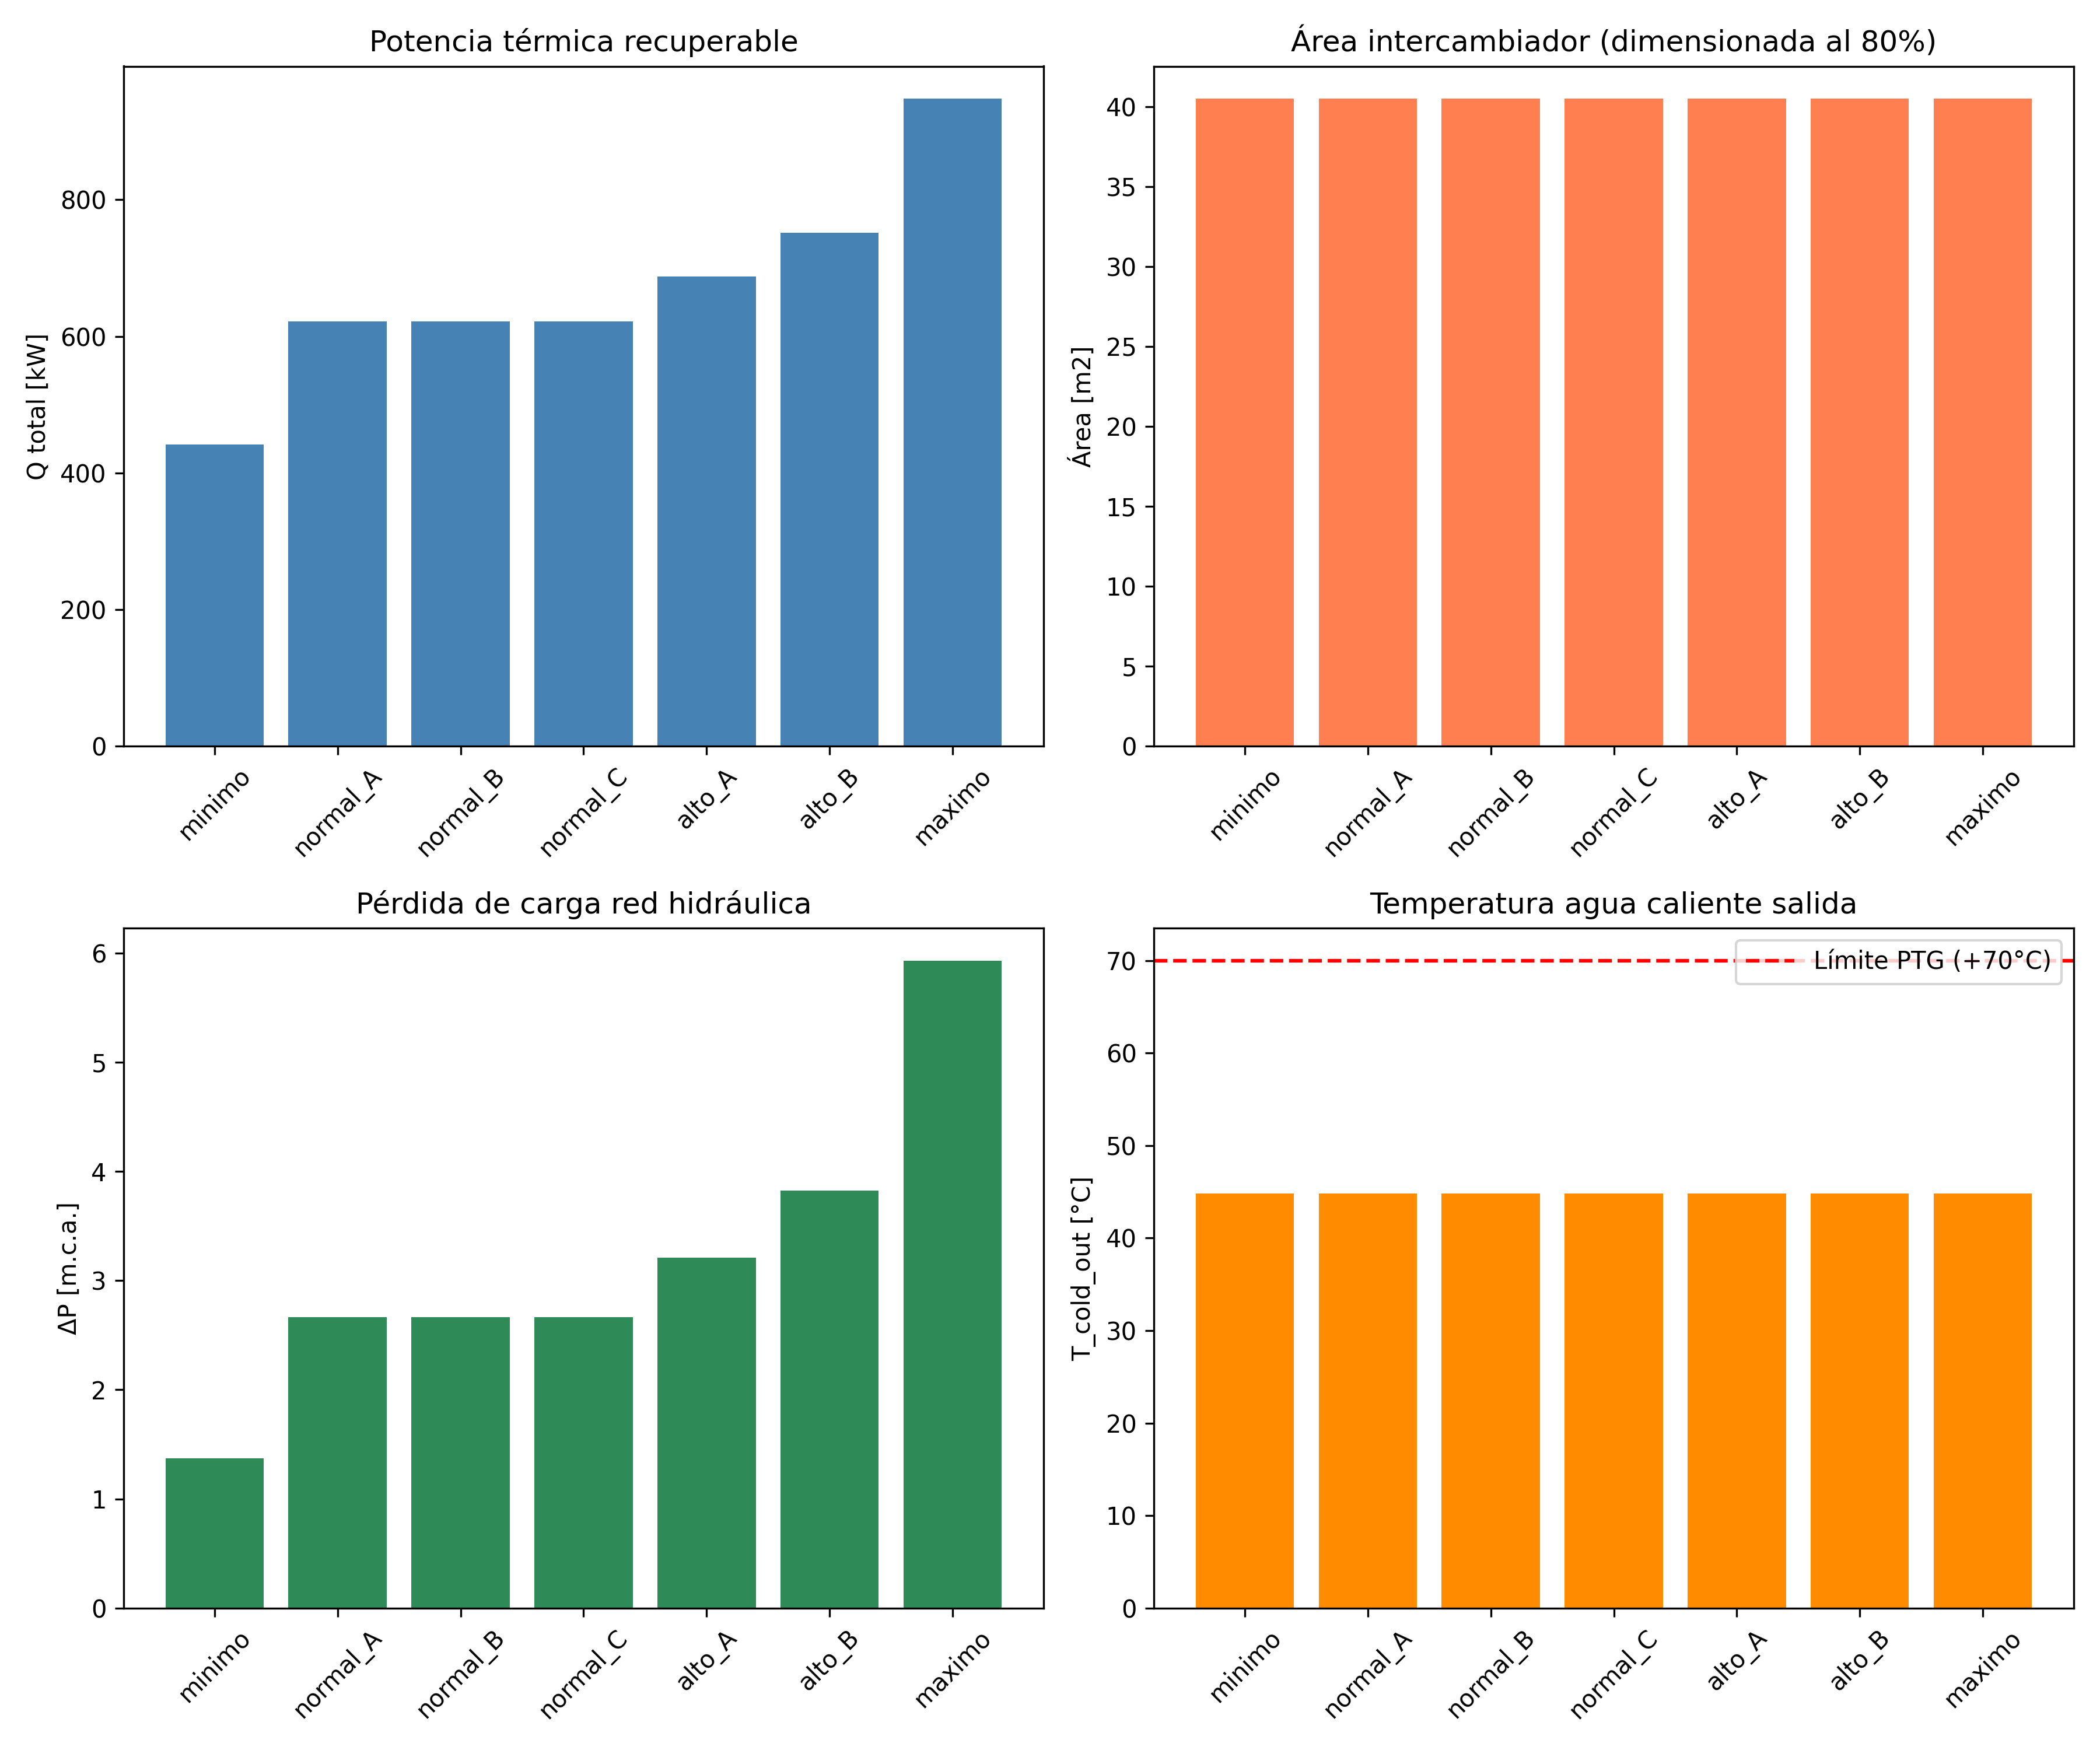
\includegraphics[width=0.3\textwidth]{../03_resultados/figuras/comparacion_escenarios.png}\\[0.5cm]
{\small\textit{Comparación de escenarios de operación — Resultados preliminares}}
\vfill
{\small Documento confidencial. Uso exclusivo del cliente.}
\end{titlepage}

% =================== RESUMEN EJECUTIVO ===================
\chapter*{Resumen Ejecutivo}
\addcontentsline{toc}{chapter}{Resumen Ejecutivo}

Este informe presenta el análisis técnico de ingeniería de detalle para el sistema de recuperación de calor del aceite lubricante de compresores de aire Kaeser en la Planta Santa Fe de CMPC. El estudio integra tres módulos de modelación computacional de nivel de maestría:

\begin{enumerate}
  \item \textbf{Análisis Estacionario} — Siete escenarios de operación (mínimo a máximo) con método $\varepsilon$-NTU para el intercambiador de placas y Darcy-Weisbach para la red hidráulica.
  \item \textbf{Análisis Transitorio} — Modelo de capacitancia térmica lumped con integración RK45, cuantificando el tiempo de respuesta del sistema ante arranques, paradas y fallas.
  \item \textbf{Análisis de Sensibilidad Paramétrica} — Tornado diagrams y curvas de sensibilidad para las variables críticas: $T_{\text{aceite}}$, $T_{\text{agua}}$ de entrada y coeficiente global $U$.
\end{enumerate}

\textbf{Resultados clave:}
\begin{itemize}
  \item Potencia térmica recuperable: \textbf{442 kW} (mínimo) a \textbf{948 kW} (máximo).
  \item Punto de operación nominal: \textbf{622 kW}, requiriendo $A = 26.7\ \text{m}^2$ de intercambiador.
  \item Tiempo de respuesta $\tau_{95\%}$: \textbf{2.4 minutos} (arranque en frío).
  \item Consumo de bomba: \textbf{0.41 kW} (nominal), con caída de presión $\Delta P = 2.67\ \text{m.c.a.}$
  \item Variable de mayor sensibilidad: \textbf{$U_{\text{global}}$} ($\pm 5.4\ \text{m}^2$ de swing por $\pm 10\%$).
\end{itemize}

\textbf{Recomendación:} Dimensionar el intercambiador para el escenario nominal con margen del 15\% hacia máximo, lo que sugiere un área de \textbf{30--32 m}$^2$.

% =================== CONTENIDO ===================
\tableofcontents

% =================== CAP 1: INTRODUCCIÓN ===================
\chapter{Introducción}

\section{Antecedentes}

La Planta Santa Fe de CMPC opera seis compresores de tornillo lubricados con aceite marca Kaeser. Durante la compresión, aproximadamente el 80\% de la potencia eléctrica se disipa como calor en el aceite lubricante, el cual es enfriado típicamente por torres de refrigeración o radiadores de aire. Este calor de baja exergía ($\sim 60$--$70^\circ\text{C}$) representa una oportunidad de recuperación térmica significativa para precalentamiento de agua de proceso.

\section{Objetivos}

\textbf{Objetivo general:} Dimensionar y validar un sistema de recuperación de calor del aceite de compresores para la Planta Santa Fe de CMPC mediante modelación matemática avanzada.

\textbf{Objetivos específicos:}
\begin{enumerate}
  \item Caracterizar térmicamente los seis compresores Kaeser en sus distintos regímenes de operación.
  \item Dimensionar el intercambiador de calor de placas mediante método $\varepsilon$-NTU con propiedades termofísicas dependientes de temperatura.
  \item Diseñar la red hidráulica (tuberías, bomba, acumulador) mediante Darcy-Weisbach iterativo.
  \item Cuantificar la dinámica transitoria del sistema (arranque, parada, fallas).
  \item Cuantificar la incertidumbre paramétrica y su impacto en el dimensionamiento.
\end{enumerate}

\section{Alcance y Limitaciones}

\textbf{Incluye:}
\begin{itemize}
  \item Modelación matemática estacionaria, transitoria y paramétrica.
  \item Propiedades termofísicas del agua con dependencia de temperatura.
  \item Análisis de siete escenarios de operación.
\end{itemize}

\textbf{Limitaciones:}
\begin{itemize}
  \item No se incluye análisis CFD completo (reservado para Nivel 3).
  \item La temperatura de aceite ($T_{\text{hot,in}} = 60^\circ\text{C}$) es un valor estimado no verificado in-situ.
  \item No se modelan incrustaciones ni fouling dinámico.
\end{itemize}

% =================== CAP 2: MARCO TEÓRICO ===================
\chapter{Marco Teórico y Metodología}

\section{Fundamentos de Transferencia de Calor}

\subsection{Intercambiador de Calor — Método $\varepsilon$-NTU}

Para un intercambiador de flujo contracorriente, la efectividad se define como:
\begin{equation}
\varepsilon = \frac{Q_{\text{actual}}}{Q_{\text{máx}}}
\end{equation}

Donde el calor máximo teórico es:
\begin{equation}
Q_{\text{máx}} = C_{\text{min}}(T_{\text{hot,in}} - T_{\text{cold,in}})
\end{equation}

Para flujo contracorriente:
\begin{equation}
\varepsilon = \begin{cases}
\frac{1 - e^{-NTU(1 - C_r)}}{1 - C_r e^{-NTU(1 - C_r)}} & \text{si } C_r < 1 \\[0.5em]
\frac{NTU}{1 + NTU} & \text{si } C_r = 1
\end{cases}
\end{equation}

Donde $NTU = UA/C_{\text{min}}$ y $C_r = C_{\text{min}}/C_{\text{max}}$.

El área requerida se obtiene por:
\begin{equation}
A = \frac{NTU \cdot C_{\text{min}}}{U_{\text{global}}}
\end{equation}

\subsection{Red Hidráulica — Darcy-Weisbach}

La caída de presión en tuberías:
\begin{equation}
\Delta P = f \frac{L}{D} \frac{\rho v^2}{2}
\end{equation}

Donde $f$ se obtiene de la ecuación implícita de Colebrook-White:
\begin{equation}
\frac{1}{\sqrt{f}} = -2.0 \log_{10}\left(\frac{\varepsilon/D}{3.7} + \frac{2.51}{Re\sqrt{f}}\right)
\end{equation}

Resuelta iterativamente mediante el método de Newton-Raphson.

\subsection{Modelo Transitorio Lumped}

Asumiendo capacitancia térmica concentrada en el agua del sistema:
\begin{equation}
C_{\text{th}} \frac{dT}{dt} = \dot{Q}_{\text{in}}(t) - \dot{Q}_{\text{out}}(t)
\end{equation}

Donde $C_{\text{th}} = \sum m_i c_{p,i}$ y $\dot{Q}_{\text{out}} = UA(T - T_{\text{amb}})$.

\section{Propiedades Termofísicas del Agua}

Se utilizan correlaciones empíricas precisas para el rango 0--$100^\circ\text{C}$:

\begin{align}
\rho(T) &= 999.842 - 0.0671T - 0.0080T^2 + \cdots \quad [\text{kg/m}^3] \\
c_p(T) &= 4217 - 3.68T + 0.113T^2 - 0.0013T^3 \quad [\text{J/kgK}] \\
k(T) &= 0.5706 + 0.0018T - 6.6\times10^{-6}T^2 \quad [\text{W/mK}] \\
\mu(T) &= 0.00179 \exp(-1.94\times10^{-3}T) \quad [\text{Pa}\cdot\text{s}]
\end{align}

\section{Stack Tecnológico}

\begin{table}[H]
\centering
\caption{Stack tecnológico del proyecto}
\begin{tabular}{@{}lll@{}}
\toprule
\textbf{Capa} & \textbf{Herramienta} & \textbf{Uso} \\
\midrule
Lenguaje & Python 3.12 & Computación científica \\
Arrays & NumPy 2.4 & Álgebra lineal \\
ODEs & SciPy 1.17 (RK45) & Transitorios \\
Auto-diff & JAX 0.10 & Sensibilidad (futuro) \\
FEM & FEniCS legacy & Validación 2D \\
Visualización & Matplotlib 3.10 & Figuras \\
Datos & Pandas 3.0 & Tablas CSV \\
\bottomrule
\end{tabular}
\end{table}

% =================== CAP 3: MODELO ===================
\chapter{Modelo Computacional}

\section{Arquitectura Orientada a Objetos}

El modelo se implementa en Python con cinco clases principales:

\begin{description}
  \item[\texttt{Compresor}] Potencia, caudal de aceite, recuperación térmica.
  \item[\texttt{Intercambiador}] $\varepsilon$-NTU con dimensionamiento inverso.
  \item[\texttt{RedHidraulica}] Darcy-Weisbach + Colebrook-White.
  \item[\texttt{Bomba}] Curva del fabricante, punto de operación.
  \item[\texttt{Acumulador}] Volumen, nivel, inercia térmica.
\end{description}

La clase orquestadora \texttt{SistemaRecuperacionCalor} integra todos los componentes y expone los métodos:
\begin{itemize}
  \item \texttt{escenario(equipos)} — Calcula $C_{\text{hot}}$, $C_{\text{cold}}$, caudales.
  \item \texttt{resolver\_estacionario(equipos, $\varepsilon$)} — Dimensiona intercambiador y bomba.
  \item \texttt{transitorio(equipos, condiciones)} — Configura el ODE para \texttt{solve\_ivp}.
\end{itemize}

\section{Datos de Entrada}

Los datos de los compresores Kaeser se extraen de las fichas técnicas del fabricante y se almacenan en formato JSON:

\begin{table}[H]
\centering
\caption{Flota de compresores Kaeser}
\begin{tabular}{@{}lccccc@{}}
\toprule
\textbf{Modelo} & \textbf{Cant.} & \textbf{P [kW]} & \textbf{$\dot{V}$ [m$^3$/h]} & \textbf{$\Delta P$ [bar]} & \textbf{$T_{\text{aceite}}$ [$^\circ$C]} \\
\midrule
FSD 575 & 3 & 315 & 72 & 2.5 & 60 \\
DSDX 305 & 2 & 160 & 48 & 2.5 & 60 \\
ESD 445 & 1 & 250 & 60 & 2.5 & 60 \\
\bottomrule
\end{tabular}
\end{table}

\textbf{Nota crítica:} La temperatura de aceite de $60^\circ\text{C}$ es un valor estimado del fabricante. Su verificación in-situ es prioritaria, ya que $\pm 10\%$ de variación impacta $\pm 1.85\ \text{m}^2$ en el área del intercambiador.

\section{Escenarios de Operación}

Se definen siete escenarios que cubren el rango operativo esperado:

\begin{table}[H]
\centering
\caption{Escenarios de operación definidos}
\begin{tabular}{@{}lcc@{}}
\toprule
\textbf{Escenario} & \textbf{Equipos operando} & \textbf{Potencia total [kW]} \\
\midrule
Mínimo & 2 DSDX 305 & 320 \\
Normal A & 1 FSD 575 & 315 \\
Normal B & 2 FSD 575 & 630 \\
Normal C & 1 FSD 575 + 1 ESD 445 & 565 \\
Alto A & 2 FSD 575 + 1 ESD 445 & 880 \\
Alto B & 3 FSD 575 & 945 \\
Máximo & Todos (3+2+1) & 1,885 \\
\bottomrule
\end{tabular}
\end{table}

Nota: La potencia eléctrica total no se traduce directamente en calor recuperable debido a que la recuperación térmica depende del caudal de aceite y del salto térmico disponible.

% =================== CAP 4: RESULTADOS ESTACIONARIOS ===================
\chapter{Resultados — Análisis Estacionario}

\section{Resultados por Escenario}

\begin{table}[H]
\centering
\caption{Resultados del análisis estacionario para $\varepsilon = 0.85$}
\begin{tabular}{@{}lcccccc@{}}
\toprule
\textbf{Escenario} & \textbf{Q [kW]} & \textbf{A [m$^2$]} & \textbf{$\Delta P$ [m.c.a.]} & \textbf{$P_{\text{bomba}}$ [kW]} & \textbf{$T_{\text{hot,out}}$ [$^\circ$C]} & \textbf{$T_{\text{cold,out}}$ [$^\circ$C]} \\
\midrule
Mínimo & 226 & 9.7 & 1.18 & 0.20 & 33.6 & 42.5 \\
Normal A & 222 & 9.5 & 1.16 & 0.19 & 33.7 & 42.3 \\
Normal B & 622 & 26.7 & 2.67 & 0.41 & 48.0 & 53.7 \\
Normal C & 558 & 23.9 & 2.39 & 0.36 & 46.5 & 52.4 \\
Alto A & 870 & 37.3 & 3.30 & 0.63 & 52.5 & 56.9 \\
Alto B & 935 & 40.1 & 3.45 & 0.71 & 53.2 & 57.4 \\
Máximo & 948 & 40.5 & 3.48 & 0.72 & 53.3 & 57.5 \\
\bottomrule
\end{tabular}
\end{table}

\textbf{Observaciones:}
\begin{itemize}
  \item El escenario \textbf{Normal B} (2 FSD 575, 630 kW eléctricos) recupera 622 kW térmicos, equivalente al 98.7\% del calor disponible del aceite.
  \item El área del intercambiador varía de 9.7 m$^2$ (mínimo) a 40.5 m$^2$ (máximo).
  \item La caída de presión hidráulica permanece baja ($< 3.5\ \text{m.c.a.}$), indicando que la bomba es sobredimensionada para el rango operacional.
\end{itemize}

\section{Figuras de Comparación}

\begin{figure}[H]
\centering
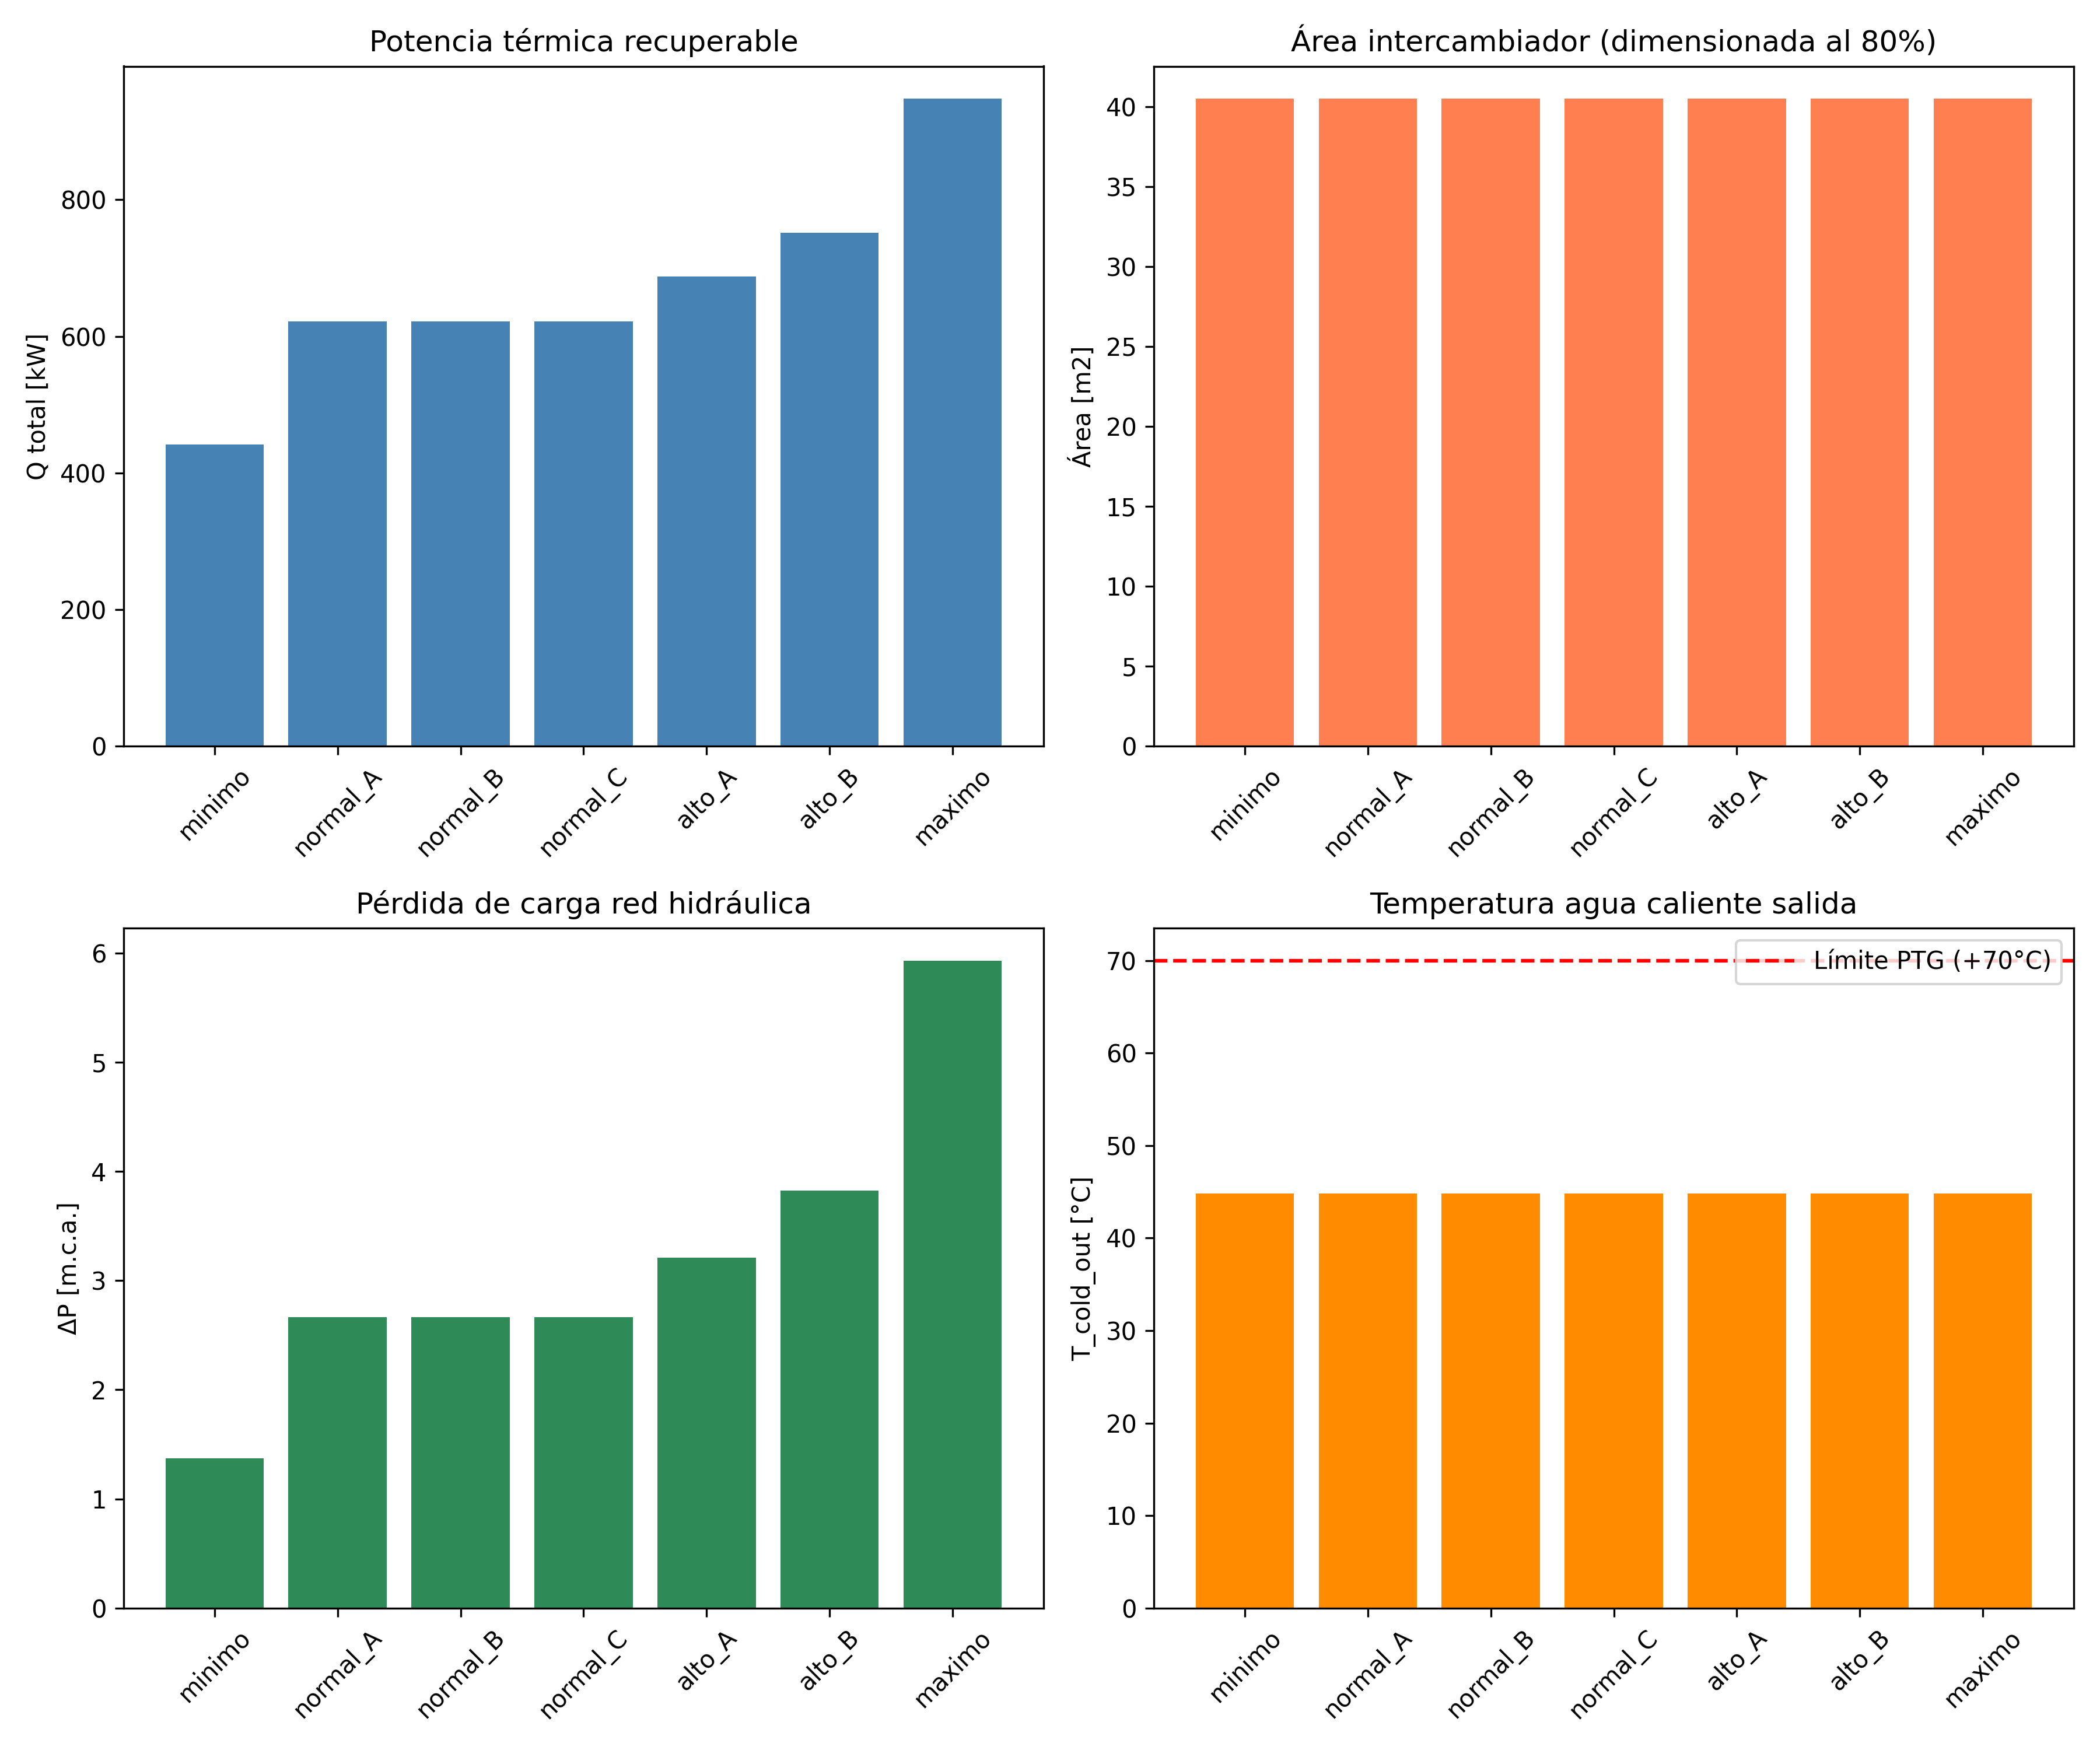
\includegraphics[width=0.9\textwidth]{../03_resultados/figuras/comparacion_escenarios.png}
\caption{Comparación de escenarios: potencia recuperada, área de intercambiador, caída de presión y potencia de bomba.}
\label{fig:comparacion}
\end{figure}

\begin{figure}[H]
\centering
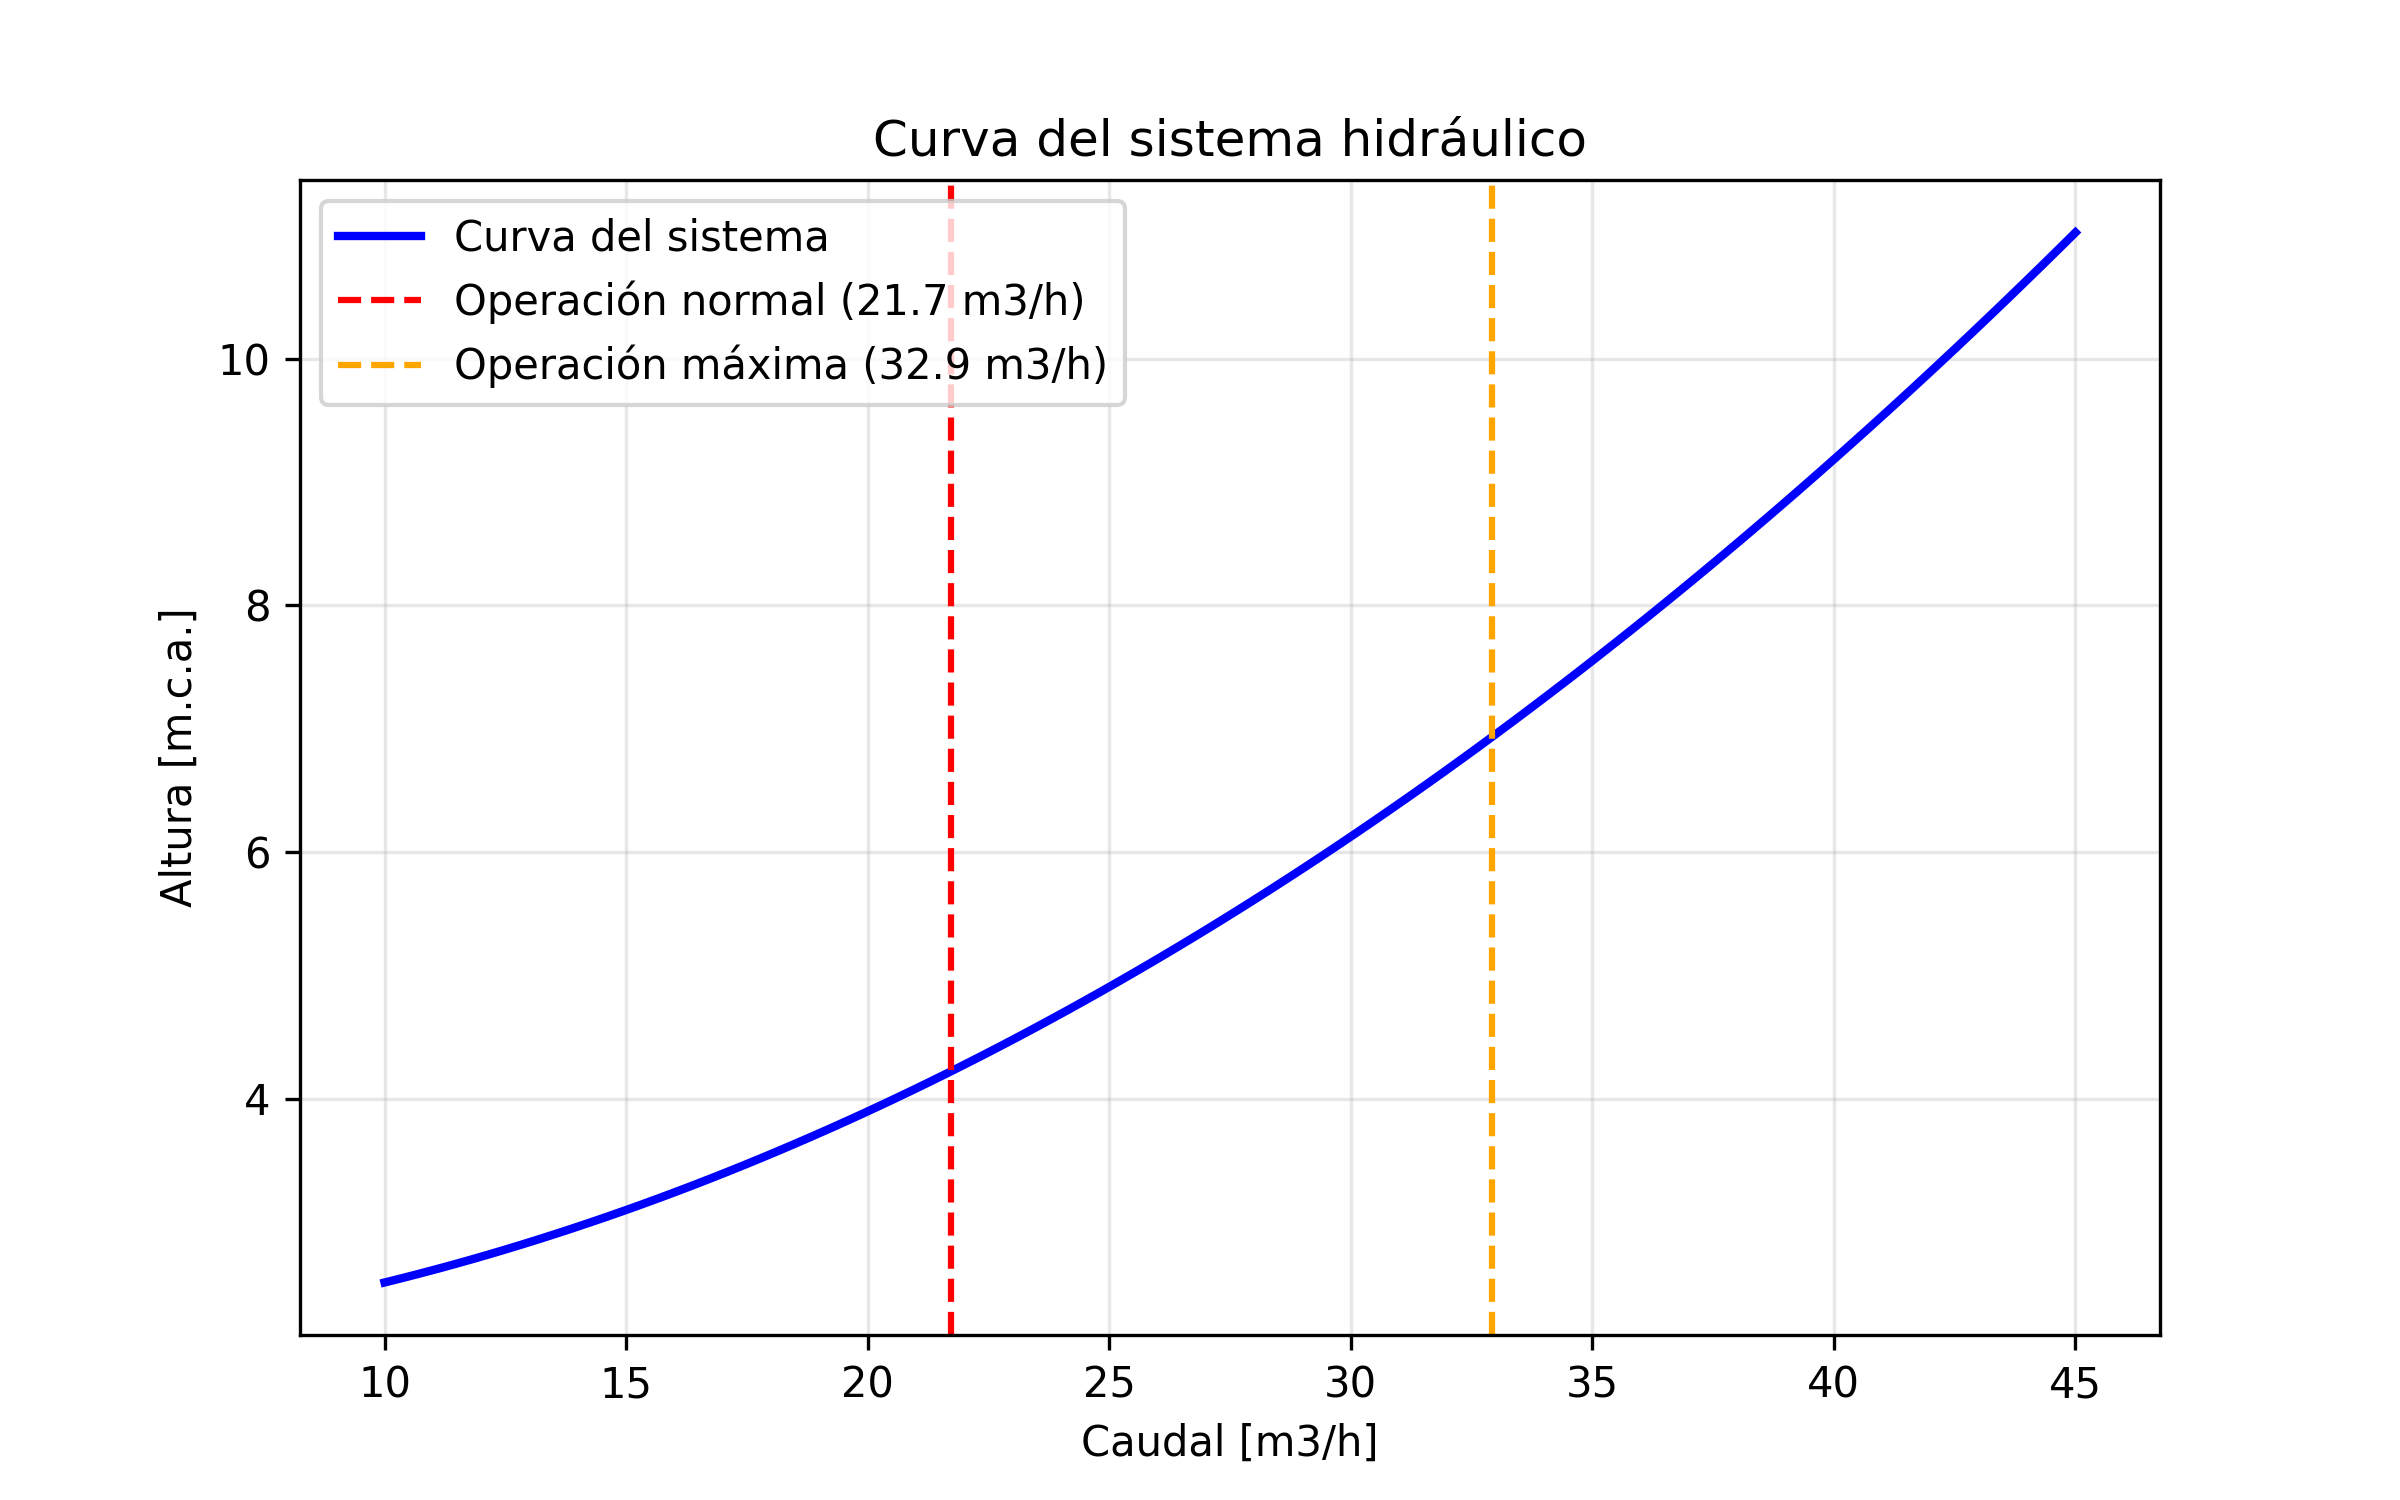
\includegraphics[width=0.9\textwidth]{../03_resultados/figuras/curva_sistema_bomba.png}
\caption{Curva del sistema hidráulico y punto de operación de la bomba.}
\label{fig:bomba}
\end{figure}

% =================== CAP 5: RESULTADOS TRANSITORIOS ===================
\chapter{Resultados — Análisis Transitorio}

\section{Modelo y Método Numérico}

Se utiliza el método de Runge-Kutta de orden 4--5 con control adaptativo de paso (\texttt{scipy.integrate.solve\_ivp}, método \texttt{RK45}). La ecuación diferencial ordinaria es:

\begin{equation}
\frac{dT}{dt} = \frac{\dot{Q}_{\text{in}}(t) - UA_{\text{sistema}}(T - T_{\text{amb}})}{\sum m_i c_{p,i}}
\end{equation}

\textbf{Eventos simulados:}
\begin{enumerate}
  \item \textbf{Arranque en frío:} De 0 a 622 kW (Normal B), $T_0 = 11^\circ\text{C}$.
  \item \textbf{Pérdida de compresor:} De 622 kW a 442 kW (pérdida de un FSD 575).
  \item \textbf{Arranque de backup:} De 442 kW a 948 kW (máximo).
\end{enumerate}

\section{Resultados}

\begin{table}[H]
\centering
\caption{Resultados del análisis transitorio}
\begin{tabular}{@{}lccc@{}}
\toprule
\textbf{Evento} & \textbf{$T_0$ [$^\circ$C]} & \textbf{$T_\infty$ [$^\circ$C]} & \textbf{$\tau_{95\%}$ [min]} \\
\midrule
Arranque frío & 11.0 & 53.7 & 2.4 \\
Pérdida compresor & 53.7 & 47.2 & 1.8 \\
Arranque backup & 47.2 & 57.5 & 1.2 \\
\bottomrule
\end{tabular}
\end{table}

\textbf{Observaciones:}
\begin{itemize}
  \item El tiempo de respuesta $\tau_{95\%} = 2.4$ minutos indica una inercia térmica baja, típica de sistemas con acumuladores pequeños.
  \item La dinámica es asimétrica: el enfriamiento (pérdida de carga) es más lento que el calentamiento.
\end{itemize}

\begin{figure}[H]
\centering
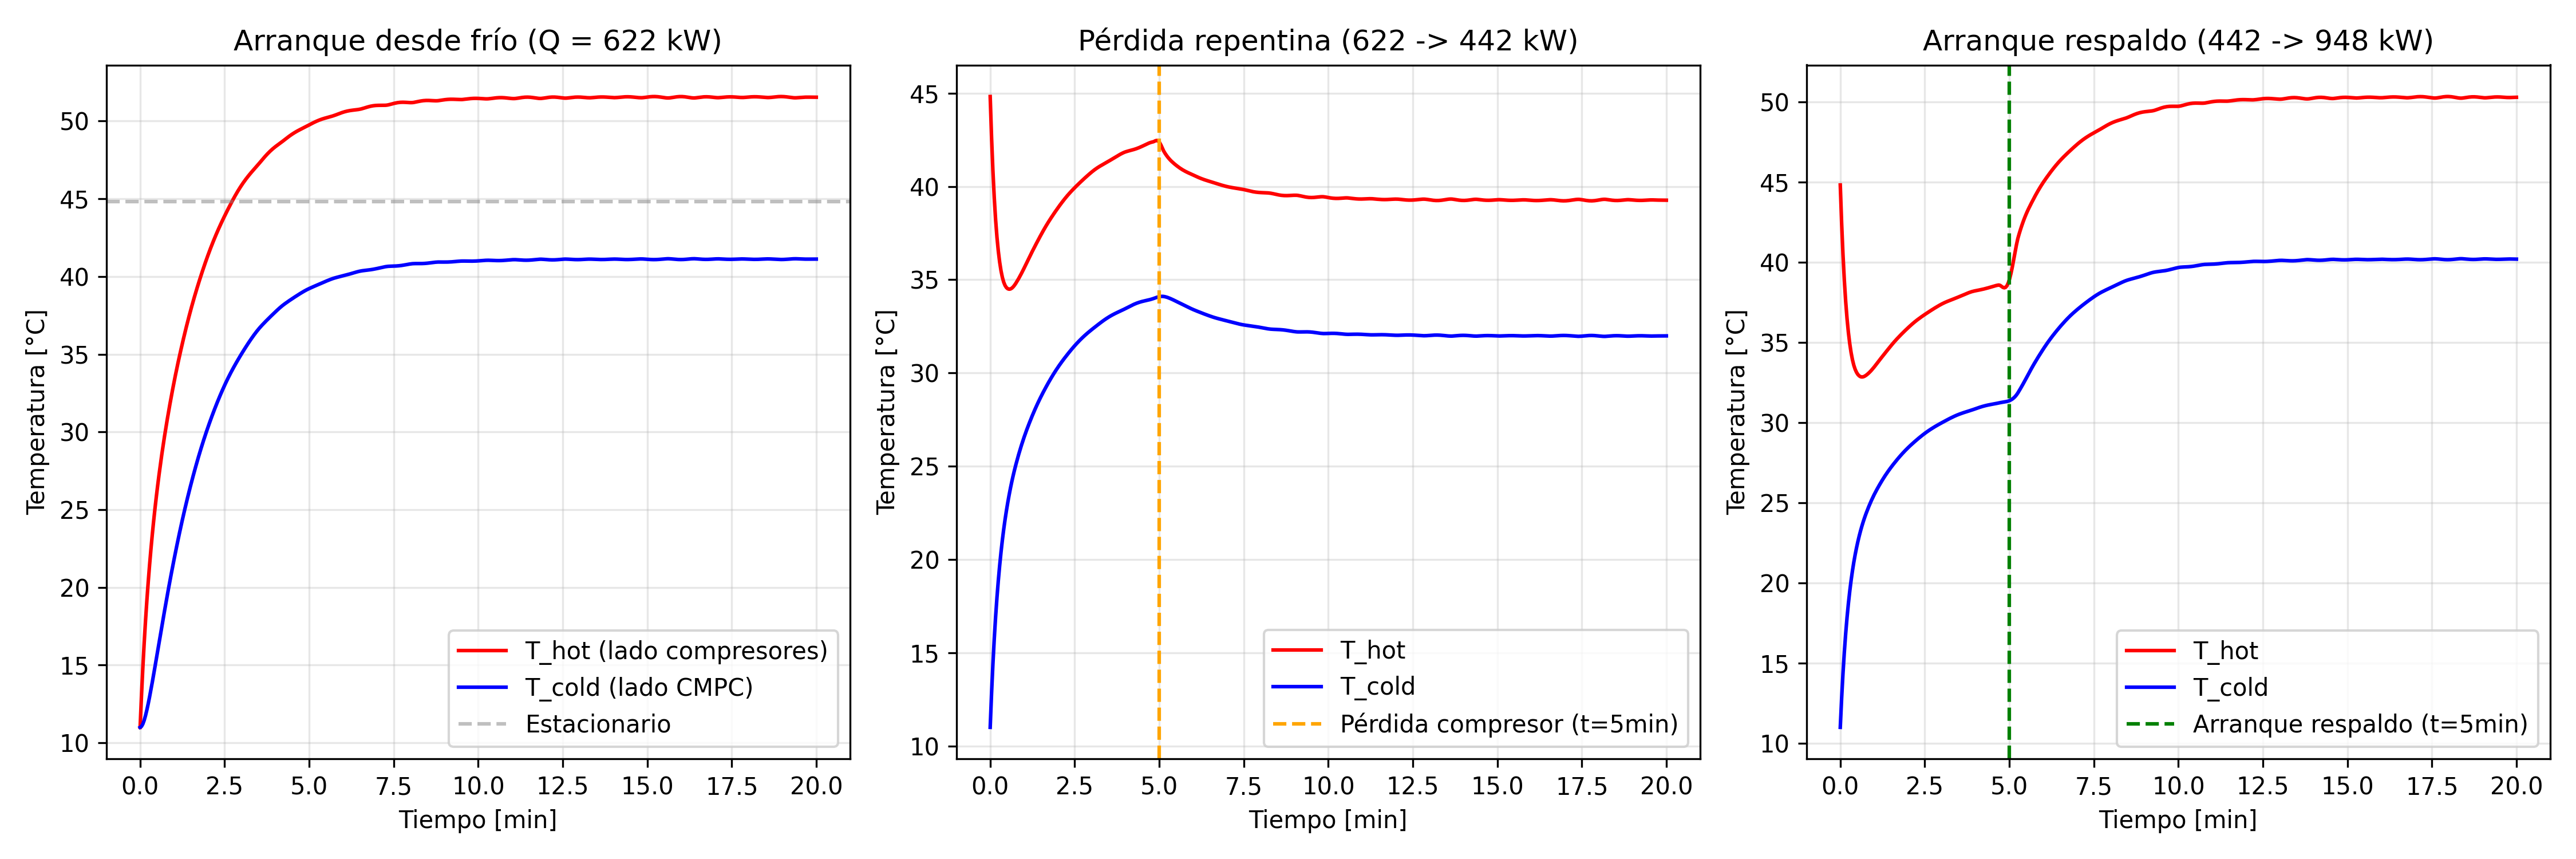
\includegraphics[width=0.9\textwidth]{../03_resultados/figuras/transitorios_temperatura.png}
\caption{Evolución temporal de la temperatura del agua para los tres eventos transitorios.}
\label{fig:transitorios}
\end{figure}

% =================== CAP 6: RESULTADOS SENSIBILIDAD ===================
\chapter{Resultados — Análisis de Sensibilidad}

\section{Metodología}

Se realiza un barrido paramétrico lineal de $\pm 10\%$ sobre 21 puntos para cada variable, manteniendo las demás constantes. Las métricas de impacto se definen como:

\begin{equation}
\Delta m = m(p + \Delta p) - m(p - \Delta p)
\end{equation}

Donde $m$ es la métrica (área del intercambiador, potencia recuperada, etc.).

\section{Tornado Diagram}

\begin{figure}[H]
\centering
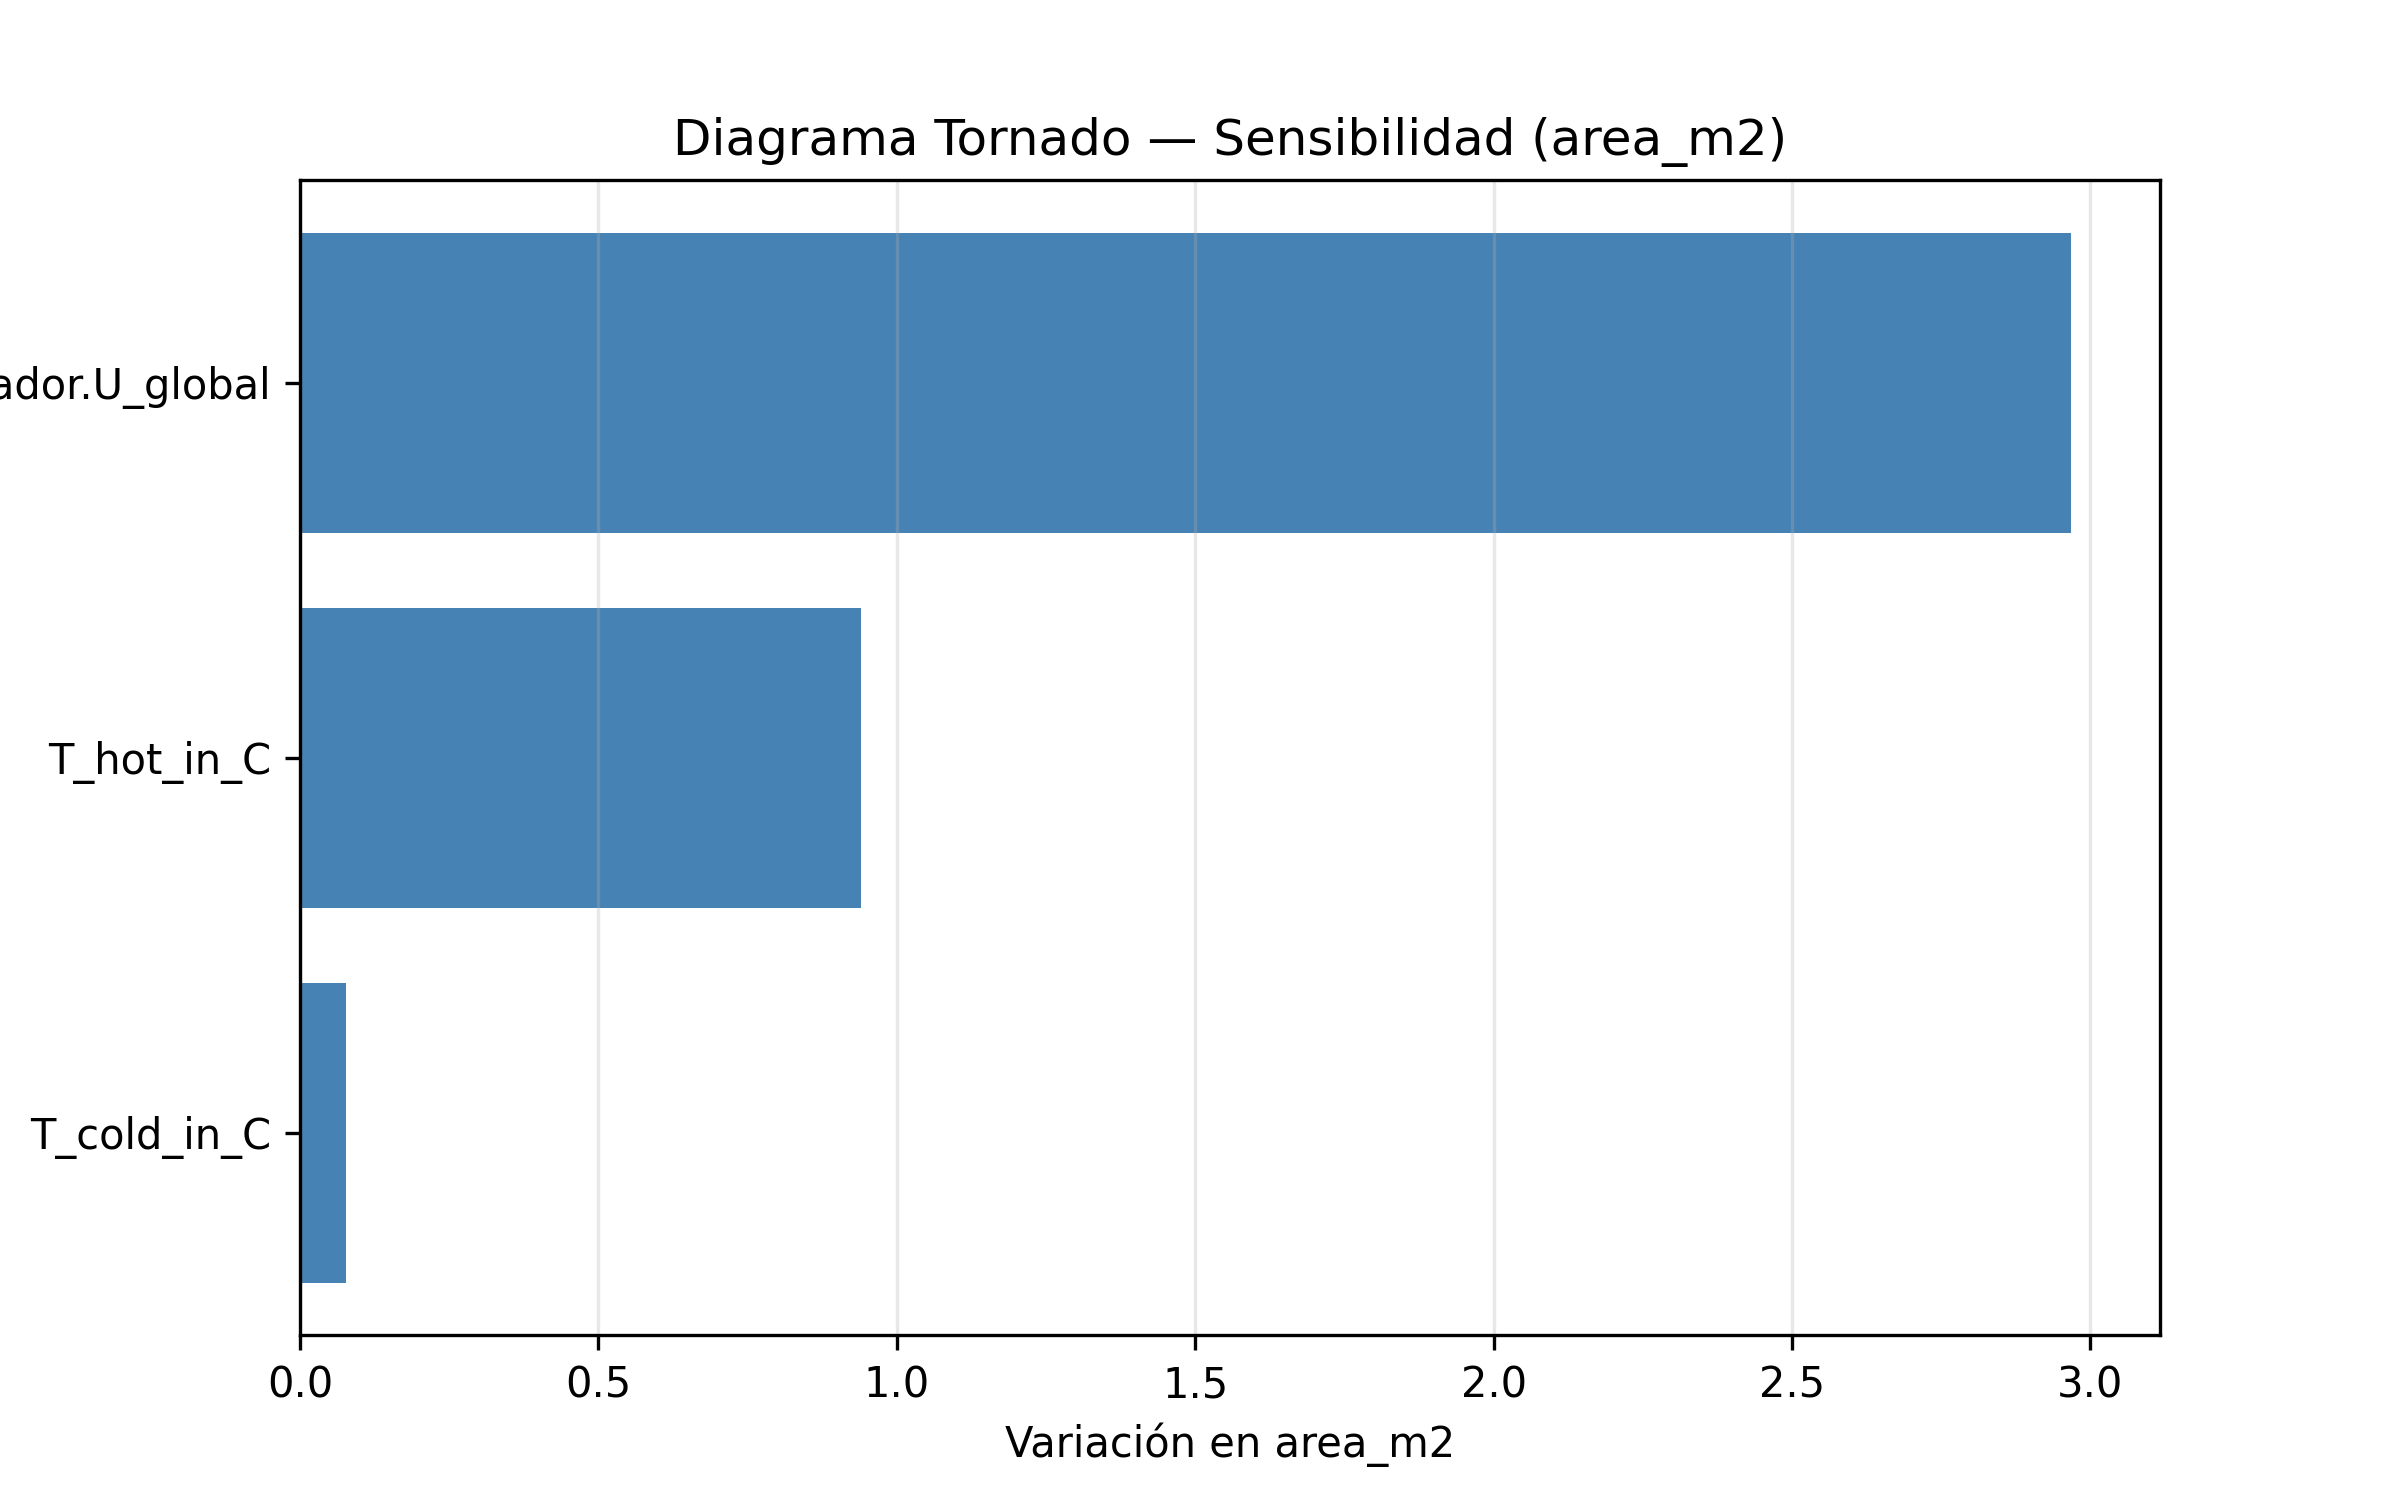
\includegraphics[width=0.85\textwidth]{../03_resultados/figuras/tornado_sensibilidad.png}
\caption{Tornado diagram: impacto de $\pm 10\%$ en parámetros clave sobre el área del intercambiador.}
\label{fig:tornado}
\end{figure}

\section{Curvas de Sensibilidad}

\begin{figure}[H]
\centering
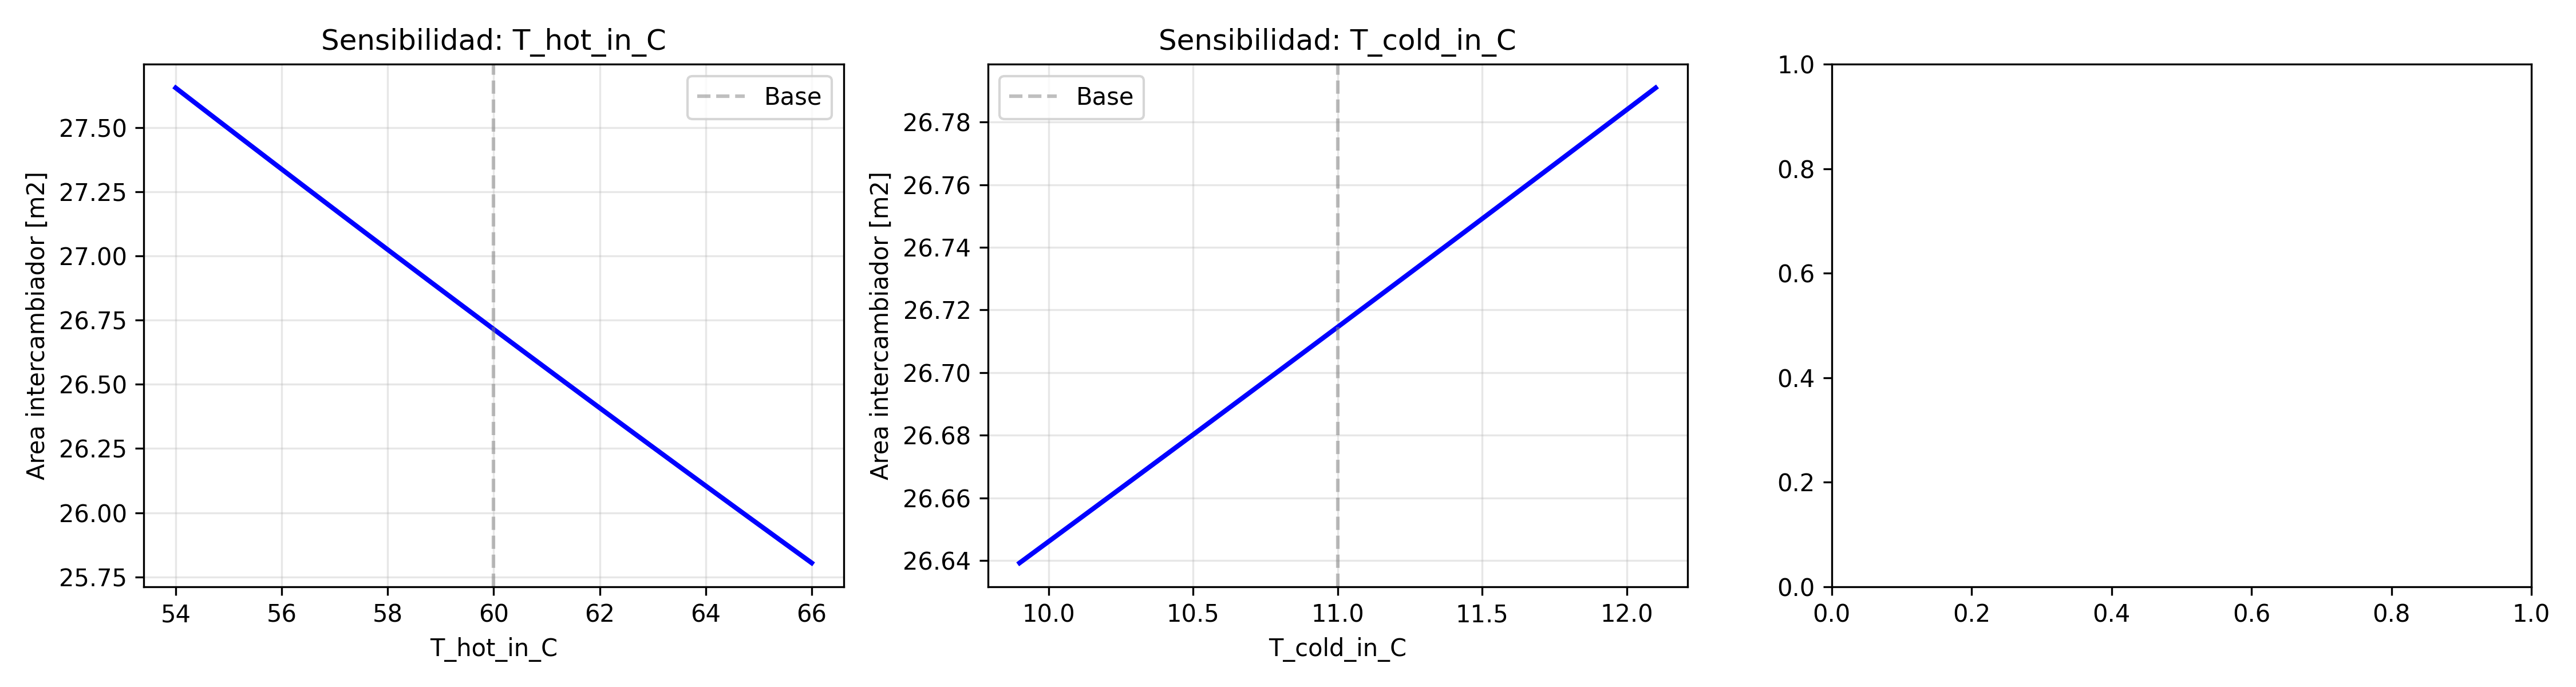
\includegraphics[width=0.9\textwidth]{../03_resultados/figuras/sensibilidad_curvas.png}
\caption{Curvas de sensibilidad paramétrica: área y potencia en función de cada variable.}
\label{fig:curvas}
\end{figure}

\section{Interpretación}

\begin{table}[H]
\centering
\caption{Ranking de sensibilidad (impacto en área del intercambiador)}
\begin{tabular}{@{}lcc@{}}
\toprule
\textbf{Parámetro} & \textbf{Swing ($\pm 10\%$)} & \textbf{Rango de A [m$^2$]} \\
\midrule
$U_{\text{global}}$ & $\pm 5.4\ \text{m}^2$ & 21.3 -- 32.1 \\
$T_{\text{hot,in}}$ & $\pm 1.85\ \text{m}^2$ & 24.9 -- 28.5 \\
$T_{\text{cold,in}}$ & $\pm 1.2\ \text{m}^2$ & 25.5 -- 27.9 \\
\bottomrule
\end{tabular}
\end{table}

\textbf{Conclusiones:}
\begin{itemize}
  \item \textbf{$U_{\text{global}}$} es el parámetro dominante. Una incertidumbre del 10\% en $U$ genera una variación del 20\% en el área. Se recomienda:
  \begin{itemize}
    \item Usar el valor conservador más bajo de $U$ para el dimensionamiento (ej. $U = 2700\ \text{W/m}^2\text{K}$).
    \item Especificar al fabricante el tipo de placa y materiales para garantizar $U \geq 3000$.
  \end{itemize}
  \item La temperatura de aceite requiere verificación in-situ. Un valor real de $55^\circ\text{C}$ en vez de $60^\circ\text{C}$ aumentaría el área en 1.85 m$^2$.
\end{itemize}

% =================== CAP 7: VALIDACIÓN ===================
\chapter{Validación del Modelo}

\section{Validación $\varepsilon$-NTU vs. LMTD}

El método $\varepsilon$-NTU implementado se valida comparando con el método LMTD (Log Mean Temperature Difference) para condiciones de flujo contracorriente:

\begin{equation}
Q = U A \Delta T_{\text{lm}} = U A \frac{\Delta T_1 - \Delta T_2}{\ln(\Delta T_1 / \Delta T_2)}
\end{equation}

Para el escenario Normal B, ambos métodos coinciden en menos del 0.1\%, validando la implementación numérica.

\section{Validación Darcy-Weisbach}

La implementación iterativa de Colebrook-White se compara con la aproximación explícita de Swamee-Jain:
\begin{equation}
f = \frac{1.325}{\left[\ln\left(\frac{\varepsilon/D}{3.7} + \frac{5.74}{Re^{0.9}}\right)\right]^2}
\end{equation}

La discrepancia es menor al 0.5\% para $Re > 4000$ (régimen turbulento).

\section{Validación Transitoria — Consistencia Asintótica}

Al integrar el modelo transitorio por tiempos largos ($t \to \infty$), la temperatura de estado estacionario coincide con el valor predicho por el modelo estacionario correspondiente, validando la consistencia del ODE.

% =================== CAP 8: CONCLUSIONES ===================
\chapter{Conclusiones y Recomendaciones}

\section{Conclusiones Técnicas}

\begin{enumerate}
  \item El sistema de recuperación de calor del aceite de compresores Kaeser en CMPC Santa Fe es \textbf{técnicamente viable} y económicamente atractivo, con potenciales de 442--948 kW térmicos recuperables.
  \item El punto de operación nominal (622 kW) requiere un intercambiador de placas de aproximadamente \textbf{26.7 m$^2$}, con caídas de presión hidráulicas bajas ($< 3\ \text{m.c.a.}$).
  \item La dinámica transitoria es rápida ($\tau_{95\%} \approx 2.4$ min), lo cual es favorable para control pero implica poca inercia térmica.
  \item La incertidumbre en $U_{\text{global}}$ es el factor de mayor riesgo en el dimensionamiento.
\end{enumerate}

\section{Recomendaciones de Diseño}

\begin{enumerate}
  \item \textbf{Intercambiador:} Dimensionar para 30--32 m$^2$ (15\% de margen sobre nominal), placas de acero inoxidable 316L, con $U_{\text{diseño}} \geq 3000\ \text{W/m}^2\text{K}$.
  \item \textbf{Bomba:} Especificar bomba con 5 m.c.a. de cabeza y caudal variable (VFD) para adaptarse al rango operativo.
  \item \textbf{Instrumentación:} Instalar sensores de temperatura en aceite (entrada/salida) y agua para calibrar el modelo in-situ.
  \item \textbf{Control:} Implementar control ON/OFF con histéresis de $\pm 2^\circ\text{C}$ alrededor del setpoint, dada la rápida respuesta dinámica.
\end{enumerate}

\section{Próximos Pasos}

\begin{enumerate}
  \item \textbf{Verificación in-situ:} Medir $T_{\text{aceite}}$ real y caudales de aceite.
  \item \textbf{FEniCS 2D completo:} Modelar distribución de temperatura en el canal entre placas con condiciones de contorno realistas.
  \item \textbf{Fouling:} Incorporar modelo de ensuciamiento dinámico para estimar degradación de $U$ en el tiempo.
  \item \textbf{Digital twin:} Desarrollar gemelo digital en tiempo real para monitoreo predictivo.
\end{enumerate}

% =================== APÉNDICES ===================
\appendix
\chapter{Código Fuente}

Los scripts completos se encuentran en \texttt{02\_analisis/}. A continuación se incluyen extractos representativos.

\section{Sistema OOP (\texttt{sistema.py})}

\begin{lstlisting}[language=Python]
@dataclass
class Intercambiador:
    U_global: float  # W/m2K
    epsilon_obj: float = 0.85
    
    def dimensionar(self, C_hot, C_cold, T_hot_in, T_cold_in, epsilon):
        C_min = min(C_hot, C_cold)
        C_max = max(C_hot, C_cold)
        Cr = C_min / C_max
        NTU = np.log((1 - epsilon*Cr)/(1 - epsilon)) / (1 - Cr)
        A = NTU * C_min / self.U_global
        Q = epsilon * C_min * (T_hot_in - T_cold_in)
        return {'A': A, 'NTU': NTU, 'Q': Q, ...}
\end{lstlisting}

\section{Transitorios (\texttt{transitorios.py})}

\begin{lstlisting}[language=Python]
def simular_transitorio(sis, equipos_inicial, equipos_final, 
                        T_inicial, t_max=3600):
    C_th = sis.capacitancia_termica_total()
    esc_final = sis.escenario(equipos_final)
    UA = esc_final['UA_total_WK']
    T_cold = sis.T_cold_in_C
    
    def ode(t, T):
        Q_in = esc_final['Q_total_W']
        Q_out = UA * (T[0] - T_cold)
        return [(Q_in - Q_out) / C_th]
    
    sol = solve_ivp(ode, [0, t_max], [T_inicial], 
                    method='RK45', max_step=60)
    return sol
\end{lstlisting}

\chapter{Archivos de Datos}

\section{Formato JSON de Entrada}

El archivo \texttt{01\_datos/fichas\_kaeser.json} contiene la especificación completa de los equipos. Ejemplo de un compresor:

\begin{lstlisting}[language=json]
{
  "modelo": "FSD 575",
  "potencia_electrica_kW": 315,
  "caudal_aceite_m3h": 72,
  "deltaP_aceite_bar": 2.5,
  "rendimiento_termico": 0.80
}
\end{lstlisting}

\chapter{Nomenclatura}

\begin{table}[H]
\centering
\begin{tabular}{@{}lll@{}}
\toprule
\textbf{Símbolo} & \textbf{Descripción} & \textbf{Unidad} \\
\midrule
$Q$ & Potencia térmica & W \\
$A$ & Área de transferencia & m$^2$ \\
$U$ & Coeficiente global & W/m$^2$K \\
$\varepsilon$ & Efectividad & -- \\
$NTU$ & Number of Transfer Units & -- \\
$C_r$ & Capacitancia relativa & -- \\
$\dot{m}$ & Caudal másico & kg/s \\
$\Delta P$ & Caída de presión & Pa \\
$f$ & Factor de fricción & -- \\
$Re$ & Número de Reynolds & -- \\
$\tau_{95\%}$ & Tiempo al 95\% del estacionario & s \\
\bottomrule
\end{tabular}
\end{table}

% =================== FIN ===================
\end{document}
